
\chapter{Running a tournament}

\section{Interpreters}

The remaining games after detecting equivalences must be played
quickly to be able to get a result in an acceptable time frame.
I implemented two \emph{interpreters} for Platypus matches, one which
uses scalar code and one which uses SIMD code. Both may be parallelised
over multiple cores. The interpreters are implemented in the file
\texttt{Code/run-game.lisp}.

The interpreters play a member of each \emph{equivalence set} produced
by equivalence detection, rather than playing every possible player
against another. Thus the points and win achieved from a match must
be weighted by the size of the equivalence set of the opponent, as one
such match is being performed in place of a match for each member
of the opposing equivalence set. For example, if Player 1 scores $10$ points
against a Player 2 chosen from an equivalence set of $2^{20}$ machines,
$10 \times 2^{20}$ points must be added to the total score of Player 1.

\subsection{Naïve interpreter}

The na\"ive interpreter runs one match on each core. The board is also
represented as an integer (with each bit representing a cell of the board)
to avoid accessing memory.

\subsection{SIMD interpreter}

The SIMD interpreter runs eight matches at once, one in each 32-bit lane
of the 256-bit operands used in operations in the \emph{Advanced Vector
  Extensions 2} (AVX2) instruction set. The interpreter works by playing
all games with one player set to the same player, and the other player
being read from the array of players. The wins and points accumulated
by games are counted in each lane. Running each match is relatively
simple, as all data used by the Platypus game can fit into 32-bit lanes,
and AVX2 provides all of the operations needed to run a Platypus game.

One issue with running a tournament in a SIMD manner is that
games vary in how long they take to complete: some finish after just
a few turns, and some run the full 50 turns. A simple use of SIMD would
be to run a game in each lane, and wait until all games finish. But
waiting for all games in all lanes to finish could thus be inefficient,
if a longer game in one lane prevents the other lanes from being
\emph{refilled}. Such a situation with 8 games played using 4 lanes is
depicted in Figure~\ref{fig:refill-all-policy}. Another simple use would be
to wait until some number of games finish and then use scalar code to
refill each lane, but the scalar code can easily become a bottleneck.

\newcommand{\game}[4]{
  \draw[fill=white] (#1, #2) rectangle +(#3, 0.5);
  \node at (#1 + 0.25, #2 + 0.25) {#4};
}
\begin{figure}
  \begin{subfigure}[b]{\textwidth}
    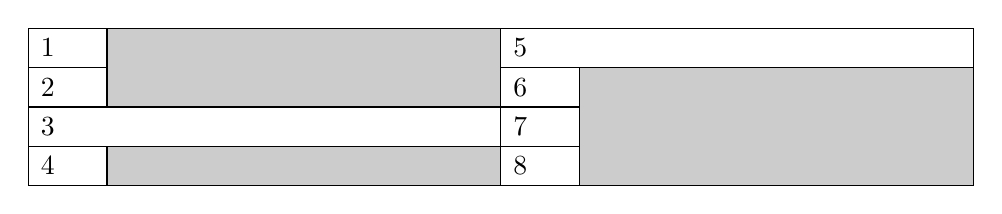
\begin{tikzpicture}
      \draw[fill=black!20!white] (0, 0) rectangle (12, 2);
      \game{0}{1.5}{1}{1}
      \game{0}{1}{1}{2}
      \game{0}{0.5}{6}{3}
      \game{0}{0}{1}{4}
      \game{6}{1.5}{6}{5}
      \game{6}{1}{1}{6}
      \game{6}{0.5}{1}{7}
      \game{6}{0}{1}{8}
    \end{tikzpicture}
    \caption{Refill when all games have finished.}
    \label{fig:refill-all-policy}
  \end{subfigure}
  
  \vspace{1em}
  
  \begin{subfigure}[b]{\textwidth}
    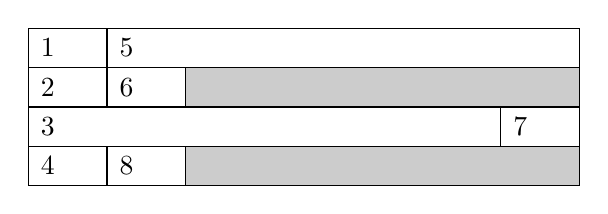
\begin{tikzpicture}
      \draw[fill=black!20!white] (0, 0) rectangle (7, 2);
      \game{0}{1.5}{1}{1}
      \game{0}{1}{1}{2}
      \game{0}{0.5}{6}{3}
      \game{0}{0}{1}{4}
      \game{1}{1.5}{6}{5}
      \game{1}{1}{1}{6}
      \game{6}{0.5}{1}{7}
      \game{1}{0}{1}{8}
    \end{tikzpicture}
    \caption{Refill when any game has finished.}
    \label{fig:refill-any-policy}
  \end{subfigure}
  \caption{How work is performed by different policies on when to refill.}
\end{figure}

Instead I manage and refill each lane individually. The SIMD interpreter
refills all lanes before taking a turn, by loading a vector of machines from
the array starting at a \emph{cursor} position, then \emph{expanding}%
\footnote{The name \emph{expand} comes from APL \cite{expand-apl}.
  Expand is implemented as an instruction in AVX-512, but AVX2
  lacks an expand instruction; so I use a lookup table to determine
  the right shuffle to do (in \texttt{+expand-table+} in \texttt{Code/vector.lisp}).}
new machines into the lanes which have finished games, and incrementing the
cursor by the number of lanes that were refilled. The tricky part of this
operation is depicted in Figure~\ref{fig:refill-algorithm}. The interpreter also
accumulates the points which the constant player acquired and
if the constant player won into counters for each lane; the 50 turns for
all $2^{28}$ machines conveniently could not possibly overflow a 32-bit
counter. Refilling each lane individually produces a work distribution
like Figure~\ref{fig:refill-any-policy}. The remaining machines are processed by
the na\"ive interpreter when there are too few remaining machines to fit into
a full\footnote{A full vector must be loaded before expansion, regardless of how
  many lanes actually get refilled.} vector. This policy provides $1.32\times$ the
throughput of refilling when all lanes are finished with 12 threads, and
$1.15\times$ the throughput with 24 threads.

\begin{figure}
  \begin{center}
    \begin{tabular}{|l|c|c|c|c|}
      \hline
      players  & 1 & 2 & 3 & 4 \\
      finished & F & T & T & F \\
      new-players & 5 & 6 & 7 & 8 \\
      \hline
      expanded := \textsc{Expand}(values: new-players, mask: finished) & \dontcare & 5 & 6 & \dontcare \\
      \textsc{Select}(mask: finished, true: expanded, false: players) & 1 & 5 & 6 & 4 \\
      \hline
    \end{tabular}
  \end{center}
  
  \caption{A state of an interpreter which needs to be refilled,
    and the SIMD operations involved in refilling the state.
    (Values we don't care about are written as \dontcare{}.)}
  \label{fig:refill-algorithm}
\end{figure}

Differential testing was again useful while implementing the SIMD
interpreter: testing should always find that the results of running games
on the na\"ive interpreter and the SIMD interpreter are be identical. In
practise testing found bugs in transitioning from SIMD code to scalar code.

\subsection{GPGPU interpreter}

A graphics processing unit (GPU) also implements a SIMD paradigm, though
typically with more lanes following the same control flow. While a GPU is
usually used to render graphics as suggested by the name, \emph{general
  purpose computing on graphics processing units} (GPGPU) interfaces like
OpenCL and CUDA allow for performing a wider range of computations on
a GPU.

I implemented the SIMD interpreter in OpenCL, though I used a more na\"ive
refilling algorithm: the program assigns small chunks of the array of
machines to lanes, and has the OpenCL implementation assign chunks to
lanes.

\section{Aggregating results}

We must aggregate the results of games from each thread somehow. Such
aggregation is complicated by a game involving two machines, and that
we need to tally the results of both machines.

One approach is to have one global table of the results of all games played
thus far. However, updating this global table requires three atomic
increments. Another approach is that each thread could instead have its
own table, and tables are only summed together when the tournament is
finished, but this arrangement would require an exorbitant amount of
space with many cores.

Another is to avoid almost all global and atomic communication by
running all games involving one machine at a time, and only update the
results pertaining to that machine. The update needn't be atomic as only
one thread will ever update the tallies for one machine. However, a thread
must play all games where a machine is used as \emph{either} player,
which ends up duplicating the work which must be performed. Guy Steele
mentions, however, that ``good parallel code often performs redundant
operations to reduce communication'' \cite{organizing-functional-code}, so
we should investigate the idea nonetheless.

A hybrid would be to partition the space of $n$ machines into disjoint
ranges, and the space of $n^2$ matches into \emph{tiles}.
Each tile consists of $(\frac{n}{t})^2$ matches for some stripe count $t$. Each
thread operates on one tile at a time, with a thread-local table of $\frac{n}{t}$
machines for either player. Updates to the global table are inherently batched
by tiling; a thread would likely have better performance by locking to update
the global table, possibly with a separate lock for each of the $t$ stripes.

I chose to use the approach which avoids all global communication.
The approach is conceptually simple, unlike the tiling approach. The approach
is also a natural fit for the SIMD interpreter, which can only easily
record results for the constant player at a time: the results for the
other player would likely to be recorded out of order, as lanes may
be refilled at any time; for example, game \#3 finishes after games \#4, \#6
and \#8 despite starting first in Figure~\ref{fig:refill-any-policy}. It is possible to
\emph{scatter} the results into a local tile in the correct locations; but this
operation is slow in practice, and scatter instructions were only introduced
in the AVX-512 instruction set extension which none of my hardware supports.

Avoiding communication is also a good fit for processors which have
many cores and relatively slow communication between cores, unlike
the global table approach. For example, the 5900X processor has a worst-case
\emph{core-to-core latency} of 84 nanoseconds
\cite{core-to-core}, which is comparable to the average time it takes to
run a Platypus match; a larger processor such as the EPYC 7773X with
64 cores has a worst-case latency of 140 nanoseconds, and the worst-case
latency of a dual-processor system may exceed 200 nanoseconds
\cite{core-to-core-2}. It would be faster to duplicate work than to pay the cost
of communication with such high latency.

It appears that atomics are also slow on the GPU; performing atomic updates
after every match was about $2.3\times$ slower than only performing updates
after completing a chunk, and thus duplicating work to avoid communication
would be faster on the GPU. However, it is possible to \emph{scatter} with good
performance on a GPU, which would permit using the tiling approach. 

\section{Benchmarks}

The benchmark measures the maximum throughput achievable by a particular
configuration of thread count and interpreter. In particular, the benchmark
must be designed to simulate the ample work provided by the full Platypus
tournament, avoiding the effects of running out of work which might be caused
by issuing a fixed amount of work. Instead my benchmark keeps all threads
running for at least a minute, and measures how long it took between starting
the benchmark and the last results being submitted, which captures the
configuration running at full throughput.

I measured the power used by each configuration using a power meter.
My desktop computer draws around 90 watts while idle with only a graphical
session and Emacs running. The results are presented in Figure~\ref{fig:benchmarks}.

\begin{figure}
  \begin{center}
    \begin{tabular}{|r r|S[table-format=4.1,mode=text] r r r|}
      \hline
      Kind & Threads & {Throughput} & Days required & Power draw & Energy required\\
           & & {(Mmatches/s)} & & (W) & (kWh) \\
      \hline
      Na\"ive & 12 & 72.6 & 947 & 184 & 4182 \\
      Na\"ive & 24 & 88.6 & 776 & 184 & 3445 \\
      SIMD & 12 & 376 & 183 & 185 & 812 \\
      SIMD & 24 & 436 & 154 & 180 & 683 \\
      GPGPU & & 1062 & 65 & 223 & 348 \\
      \hline
    \end{tabular}
  \end{center}
  \caption{The performance and energy usage of some configurations of Platypus interpreters.}
  \label{fig:benchmarks}
\end{figure}

The SIMD and GPGPU interpreters are both more energy-efficient and
faster. The SIMD interpreter does not draw more power than the na\"ive
interpreter, though intuitively performing more transitions at once
would draw more power. Guermouche and Orgerie \cite{vectorized}
examined the power draw and energy use of running various high
performance computing applications with different vector widths, and
found that the variation in power draw was dependent on the
application and the processors used; one cluster would draw 28\%
more power using 256-bit vectors instead of 128-bit vectors, but one
computer would draw the same amount of power regardless of vector
width. However, they were able to use sensors in Intel processors to
more accurately determine the power draw of the processors and
memory independently; I used an external device which measures
the power draw of the whole computer.

\section{Distribution}
\label{sec:distribution}

Another option to utilise more hardware is to distribute the tournament
across multiple computers; running the tournament is embarrasingly
parallel as there are no dependencies between Platypus games. I distributed
the tournament by separating the tournament software into a \emph{server}
which allocates work and records results into a database, and a \emph{client}
which runs work on a GPU. The server is implemented in the
\texttt{Code/Distributed-host/} directory and the client is implemented
in the \texttt{Code/OpenCL-interpreter/} directory.

The tournament is run in two phases following the communication-avoiding
technique for aggregating results, with a phase for computing the results
of matches with a machine as either player.
The client communicates with the server by making HTTP requests. The client
first downloads the arrays of machines and equivalence set sizes to play.
The client then requests some machines to test, and the client plays those
machines against all opponent machines in the arrays. Multiple machines
are issued in one request to avoid network latency: with a tournament of the
53 million unique machines we found, a client which can play one billion
matches per second would otherwise need to make a request every 19
milliseconds. The client then submits the results to be stored in the database.

The distributed architecture happens to avoid gaps in the options which AWS
offers for GPU acceleration, though I was not trying to plan around the gaps.
A g5.xlarge instance offers one GPU, four virtual CPU cores and 16 GiB of
memory, but the next largest number of GPUs is provided with a g5.12xlarge
instance with 4 GPUs, 48 CPU cores and 192 GiB of memory. I do not need the
memory or CPUs, so it is more cost effective to use a larger number of
g5.xlarge instances.

Distribution also introduces some fault-tolerance. My prior experiences with
programming for GPGPU suggested that I could easily make mistakes while
manually managing CPU and GPU memory buffers; and assigning each GPU
to a separate process would isolate errors%
\footnote{Although it is difficult to \emph{detect} memory errors in the
  first place, so this is insufficient: memory-unsafe code will only crash
  if it accesses unmapped memory, and recently deallocated
  memory and off-by-one indices tend to still be mapped.}
and allow other client processes to continue running if one fails.

\section{Heuristics}

If many matches are short, an approximation of the full tournament
results can be found by stopping matches early. The lengths of one million
random matches are shown in Figure~\ref{fig:turn-distribution}; more than half
of all matches were shorter than 10 turns long, but again coverage past that point
is more gradual, except for the 170 thousand matches which hit the turn limit.
Note also the periodic nature of the distribution: there are local maxima at 2, 12,
22 and 31 turns, possibly related to machines taking 10 turns to wrap around the
board and reach each other again.

\begin{figure}
  \begin{subfigure}[b]{0.5\textwidth}
    \centering
    \begin{tikzpicture}
      \begin{axis}[
        xlabel=Turns,
        xmin=-1, xmax=51,
        ymin=0,
        ylabel=Matches,
        width=\textwidth, height=6cm, bar width=1]
        \addplot[ybar, fill=black] table[x=turns, y=count, col sep=comma] {match-lengths.csv};
      \end{axis}
    \end{tikzpicture}
  \end{subfigure}%
  \begin{subfigure}[b]{0.5\textwidth}
    \centering
    \begin{tikzpicture}
      \begin{axis}[
        xlabel=Maximum turns,
        xmin=-1, xmax=51,
        ymin=0,
        ylabel=Matches,
        width=\textwidth, height=6cm, bar width=1]
        \addplot[mark=none] table[x=turns, y=cumulative, col sep=comma] {match-lengths.csv};
      \end{axis}
    \end{tikzpicture}
  \end{subfigure}
  \caption{The distribution of the lengths of one million random matches.}
  \label{fig:turn-distribution}
\end{figure}

Many matches take all 50 turns; if such matches do not terminate
then cutting early may still pick the machine which would win a game
with the full length. The points scored by either machine could also be
extrapolated by scaling the numbers of points, assuming that the rate
at which points are scored remains constant throughout the game.